% Auto-generated by scripts/generate_figures.py
% Insert into your LaTeX document where appropriate.

% ---- fig1_pipeline.pdf ----
\begin{figure*}[t]
  \centering
  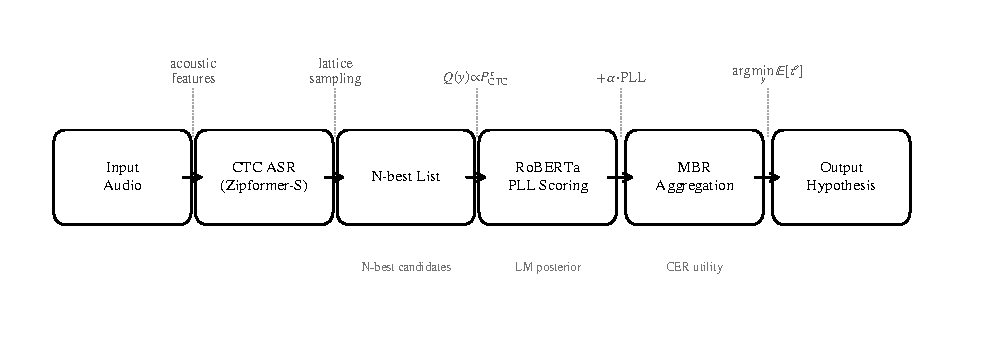
\includegraphics[width=\textwidth]{figures/fig1_pipeline.pdf}
  \caption{MBR-CER+PLL decoding pipeline. The CTC ASR model produces a $\tau$-sharpened posterior $Q(y)$ over $G$ N-best candidates via lattice sampling. RoBERTa assigns pseudo-log-likelihood (PLL) scores that augment the acoustic posterior. The MBR aggregation step selects the hypothesis minimising expected character error rate under the combined posterior.}
  \label{fig:pipeline}
\end{figure*}

% ---- fig2_gamma_split.pdf ----
\begin{figure}[t]
  \centering
  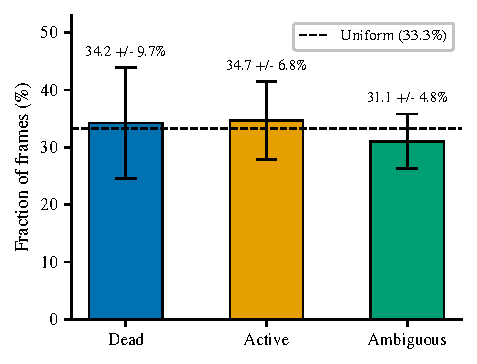
\includegraphics[width=0.46\textwidth]{figures/fig2_gamma_split.pdf}
  \caption{Three-way decomposition of CTC alignment posterior $\gamma_t$ on $n=100$ dev-other utterances. Error bars: $\pm 1$ s.d.\ across utterances. Dashed line: uniform (33.3\%). Dead and active fractions are nearly equal, contradicting the prior assumption that blank dominates ($>$70\% dead).}
  \label{fig:gamma}
\end{figure}

% ---- fig3_mwer_trajectories.pdf ----
\begin{figure*}[t]
  \centering
  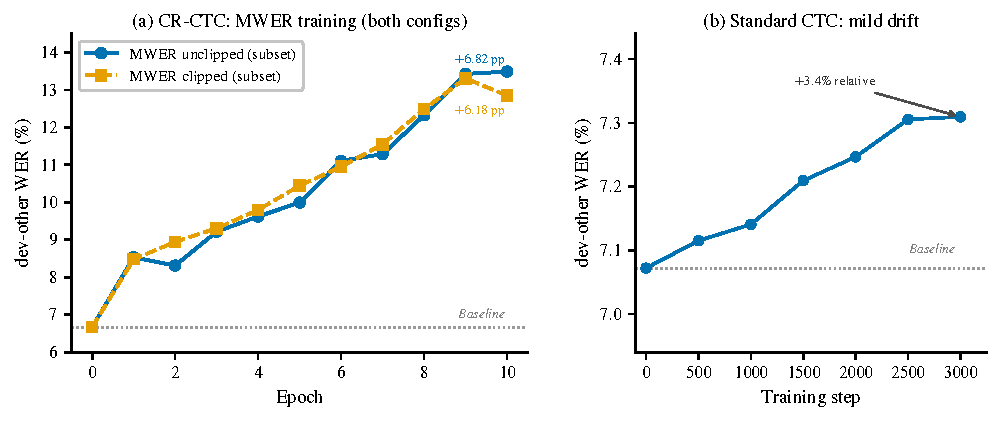
\includegraphics[width=\textwidth]{figures/fig3_mwer_trajectories.pdf}
  \caption{MWER training trajectories on dev-other. \textbf{(a)} All four CR-CTC configurations degrade monotonically. Subset configurations (MWER-unclipped-subset, MWER-clipped-subset): 248-batch subset, 10 epochs (eval at each epoch). Full-data configurations (MWER-unclipped-full, MWER-clipped-full): full training set, 1 epoch; only baseline and final eval are available (7{,}132 training steps, no intermediate dev-other checkpoints). Clipping reduces the final WER by $\approx$0.6\,pp but does not reverse degradation. \textbf{(b)} Standard CTC shows mild drift: +3.4\% relative over 3{,}000 steps.}
  \label{fig:mwer}
\end{figure*}

% ---- fig4_g_scaling.pdf ----
\begin{figure*}[t]
  \centering
  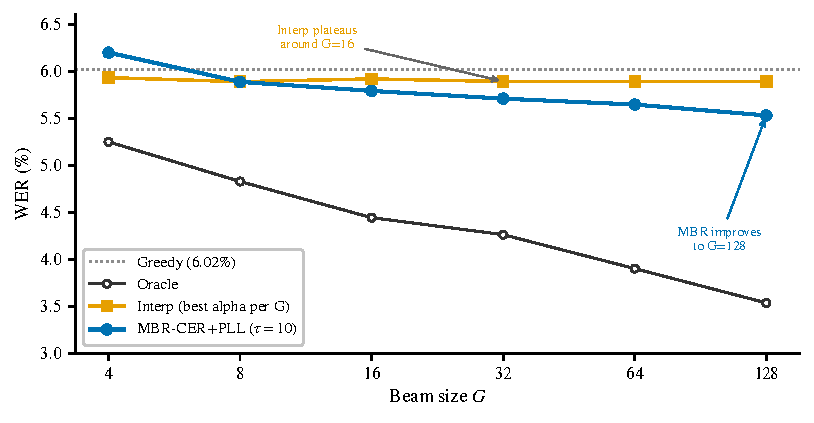
\includegraphics[width=\textwidth]{figures/fig4_g_scaling.pdf}
  \caption{WER vs beam size $G$ on dev-other. Interpolation (best $\alpha$ at each $G$) plateaus around $G=16$; MBR-CER+PLL ($\tau=10$) improves monotonically through $G=128$, closing 19.8\% of the oracle gap. See Fig.~\ref{fig:spearman} for the mechanistic explanation.}
  \label{fig:gscaling}
\end{figure*}

% ---- fig5_tau_sweep.pdf ----
\begin{figure}[t]
  \centering
  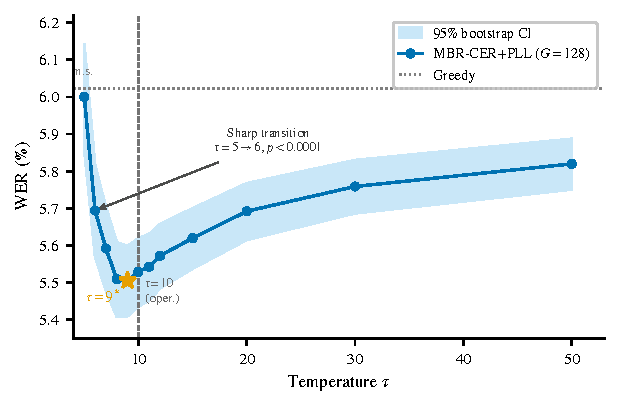
\includegraphics[width=0.46\textwidth]{figures/fig5_tau_sweep.pdf}
  \caption{WER as a function of temperature $\tau$ at $G=128$ (shaded: 95\% bootstrap CI for delta vs greedy). Sharp transition between $\tau=5$ (n.s., $p=0.38$) and $\tau=6$ ($\Delta=-0.328$\,pp, $p<0.0001$). WER is flat from $\tau=6$ to $\tau\approx15$ then degrades. Star: optimum $\tau=9$ (5.506\%); dashed: operational $\tau=10$ (5.529\%).}
  \label{fig:tau}
\end{figure}

% ---- fig6_spearman_divergence.pdf ----
\begin{figure*}[t]
  \centering
  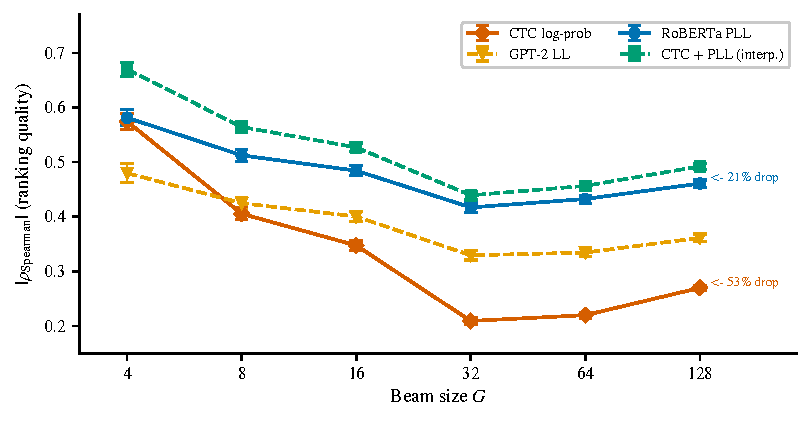
\includegraphics[width=\textwidth]{figures/fig6_spearman_divergence.pdf}
  \caption{Absolute Spearman $\rho$ between scorer and per-utterance WER vs beam size $G$ (error bars: 95\% CI). CTC log-probability degrades sharply (53\% drop, $G=4\to128$); RoBERTa PLL degrades slowly (21\% drop). This divergence explains the MBR-vs-interpolation asymmetry in Fig.~\ref{fig:gscaling}.}
  \label{fig:spearman}
\end{figure*}

% ---- fig7_cross_condition.pdf ----
\begin{figure*}[t]
  \centering
  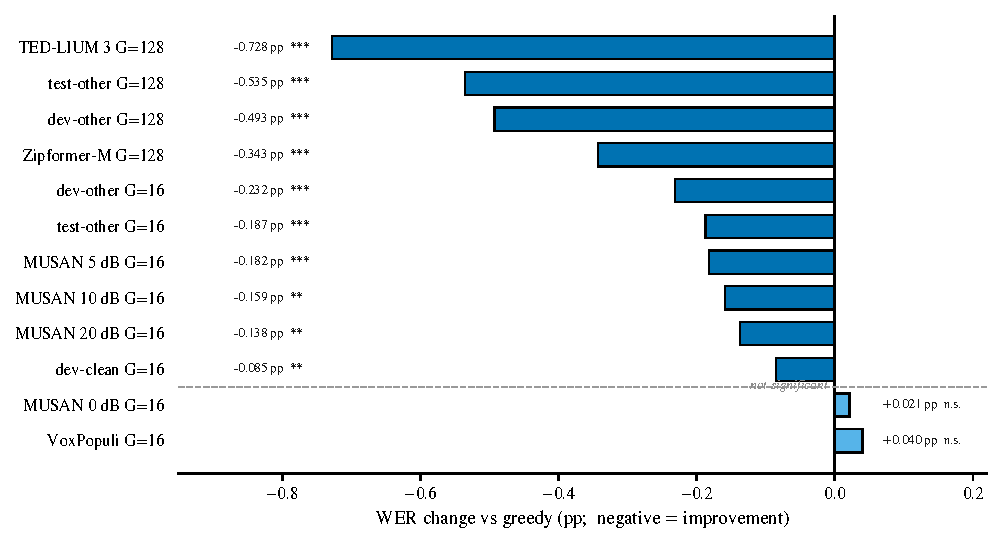
\includegraphics[width=\textwidth]{figures/fig7_cross_condition.pdf}
  \caption{WER change (MBR-CER+PLL vs greedy, pp) across all evaluation conditions. Sorted by improvement magnitude; light blue: not significant. Significance from paired bootstrap ($B=10{,}000$, seed 42): $*p<0.05$, $**p<0.01$, $***p<0.001$. VoxPopuli: coverage-bottlenecked (91.5\% of utterances already greedy-optimal, oracle gap only 0.35\,pp). MUSAN 0\,dB: candidate diversity collapses under extreme noise.}
  \label{fig:crosscond}
\end{figure*}
